\documentclass{report}

\usepackage{pgfplots}

\pgfplotsset{compat=1.6}

\begin{document}
\thispagestyle{empty}

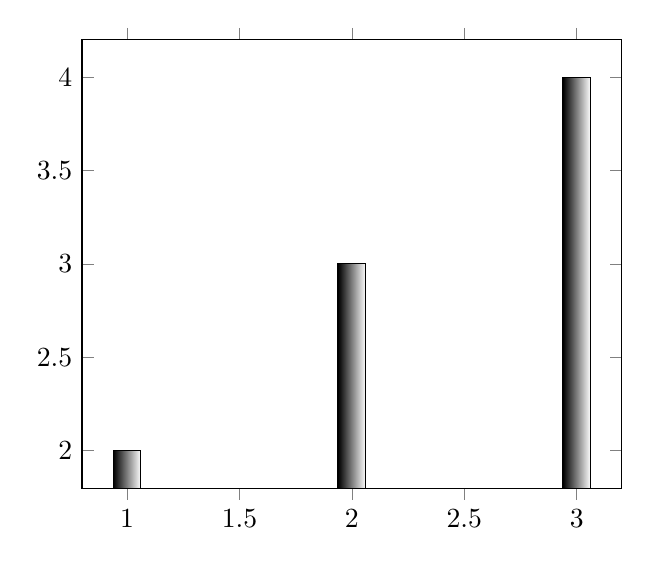
\begin{tikzpicture} 
    \begin{axis}[ybar]
        \addplot[left color=black,right color=white,
			at begin bar={%
				\begin{scope}%
				\shade\pgfextra
			},
			at end bar={%
				\endpgfextra;
				\end{scope}%
			},
		]
			coordinates {(1,2) (2,3) (3,4)}; 
    \end{axis} 
\end{tikzpicture}

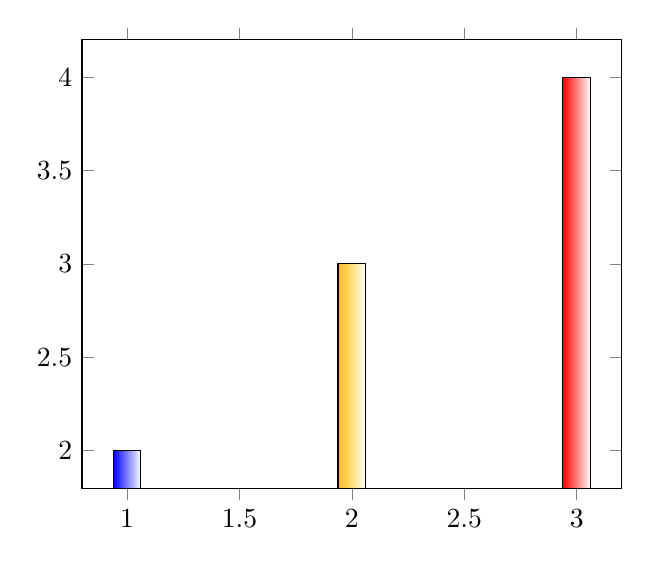
\begin{tikzpicture} 
    \begin{axis}[ybar]
        \addplot[
			point meta=x,
			at begin bar={%
				\pgfplotsaxisvisphasetransformpointmeta
				\pgfplotscolormapdefinemappedcolor{\pgfplotspointmetatransformed}%
				\begin{scope}[left color=mapped color,right color=white]%
				\shade\pgfextra
			},
			at end bar={%
				\endpgfextra;
				\end{scope}%
			},
		]
			coordinates {(1,2) (2,3) (3,4)}; 
    \end{axis} 
\end{tikzpicture}



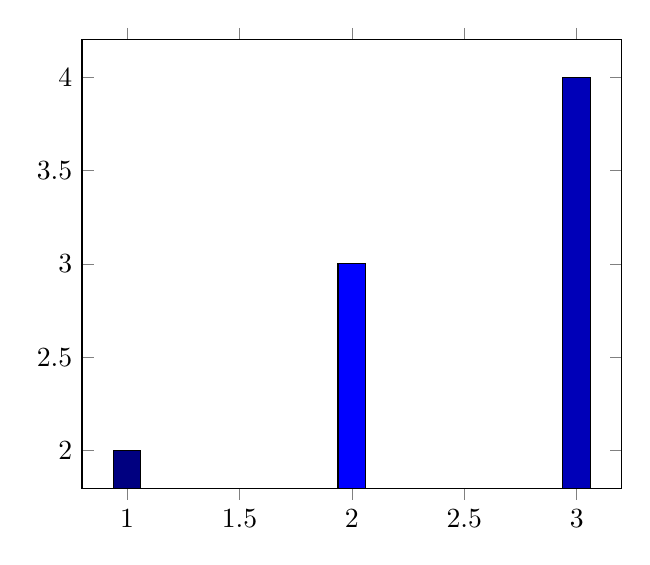
\begin{tikzpicture}
\begin{axis}[ybar]
\addplot[
	at begin bar={%
		\path[fill=blue!\cdest!black]
		\pgfextra
		% here we expect something like \pgfpathrectangle...
	},
	at end bar={%
		% this ends the preceding \pgfextra
		\endpgfextra;
	},
	visualization depends on=\thisrow{cdest}*100\as\cdest,
    ]
table {
x y cdest
1 2 0.5
2 3 1
3 4 0.72
};
\end{axis}
\end{tikzpicture}
\end{document}

